\chapter{Experiments}
In this chapter .... experiments will be presented. 
\section{Surface Accuracy on a technical phantom}
\label{sec:SurfaceReconstructionAccuracy}
The work presented in this section was presented at CURAC, Luca

Surgical resection is the gold standard for curative care for primary and
secondary hepatic tumors. This procedure usually involves removing the segment
of the liver where the tumor is located. In this treatment, it is important to
spare enough healthy parenchyma to preserve the function of the liver after
surgery. Therefore, non-anatomical resection approaches are becoming more
popular, as they try to spare as much healthy tissue as possible. This way, only
the tumor and a safety margin of 5 – 10 mm are removed which allows multiple
resections and re-treatments in case of recurrence \cite{aghayan2018laparoscopic}.
However, especially in these non-anatomical resections, maintaining the safety
margin is challenging as the tumor is removed by cutting around the tumor in a
conical or wedge shape rather than a plane along anatomical landmarks.
Therefore, image-guidance systems have been introduced to guide the surgeon to
precisely follow a planned resection path. These systems rely on tracking
devices (optical or electromagnetic) to measure the pose of the surgical
instruments and use a registration process to align a preoperative model with
the patient intraoperatively \cite{lango2012navigated}\cite{banz2016intraoperative}. However, the setup and use of such systems
is time consuming, complex and requires extensive training, which is a major
reason why they are not widely used \cite{kingham2013evolution}.
Additionally, the registration process introduces errors due to organ deformation between the image acquisition and the surgery. 
During conventional, non-anatomical resections a resection plan is drawn onto
the liver before the start of the resection. Therefore, an important part of the
resection plan is an accurate reconstruction of the liver surface. This surface
is then used to project the outline of the tumor and a safety margin onto the
surface.
This is where the surgeon would start with the transection of the parenchyma.
Previous work used such surface reconstructions based on laser scanners \cite{simpson2016current} for
intraoperative registration, which requires additional equipment.
In this study, we evaluated an ultrasound (US) based method to automatically reconstruct the liver surface intraoperatively.


\subsection{Methodology}
The image processing pipeline consists of three steps, the acquisition, the
contact detection and the surface reconstruction (Figure \ref{fig:processingPipeline}). First the data from an
ultrasound scanner (Flex focus 800, BK Medical, Denmark) and a tracking camera
(Polaris, NDI, Canada) is acquired and fused on a navigation system (CAS-One
Vario, CAScination AG, Switzerland) for liver surgery. Then each image is
classified whether it has contact to the liver surface or not. The position of
the images with contact to the liver surface are then further processed in the
surface reconstruction step to create a model of the liver surface. The result
is then visualized in a 3D viewer.
\begin{figure}[H]
  \centering
  \smartdiagram[sequence diagram]{Acquisition, Surface contact detection, Surface reconstruction}
  \caption{The data processing pipeline}
  \label{fig:processingPipeline}
\end{figure}

\subsubsection{Acquisition}
During the data acquisition phase, the ultrasound image and the corresponding 6D
pose are recorded using the navigation system. The ultrasound was calibrated
using a Z-wire phantom \cite{peterhans2010fully} and is tracked by an optical tracking system. To
simulate a liver surgery, a multimodal liver phantom (Figure \ref{fig:usedPhantom}) and an
intraoperative ultrasound was used to get the ultrasound images. During the
simulation the ultrasound device had a trackable and calibrated marker attached.
To find an optimal sampling method, the liver was scanned with six different
techniques (Figure \ref{fig:movements}). The two spiral techniques represent recordings
of moving the US device to draw a spiral onto the liver. Either from the center
to the peripheral part (spiral out) or vice versa (spiral in). The two sweep
techniques represent recordings of moving the US device left and right (Sweep
LR) or forward and backward (Sweep FB). The flower technique represents a
recording of moving the US-device to draw a flower onto the liver.
Additionally, a point grid was acquired as reference points for evaluation of
the other reconstructions.

\begin{figure}[H]
  \centering
 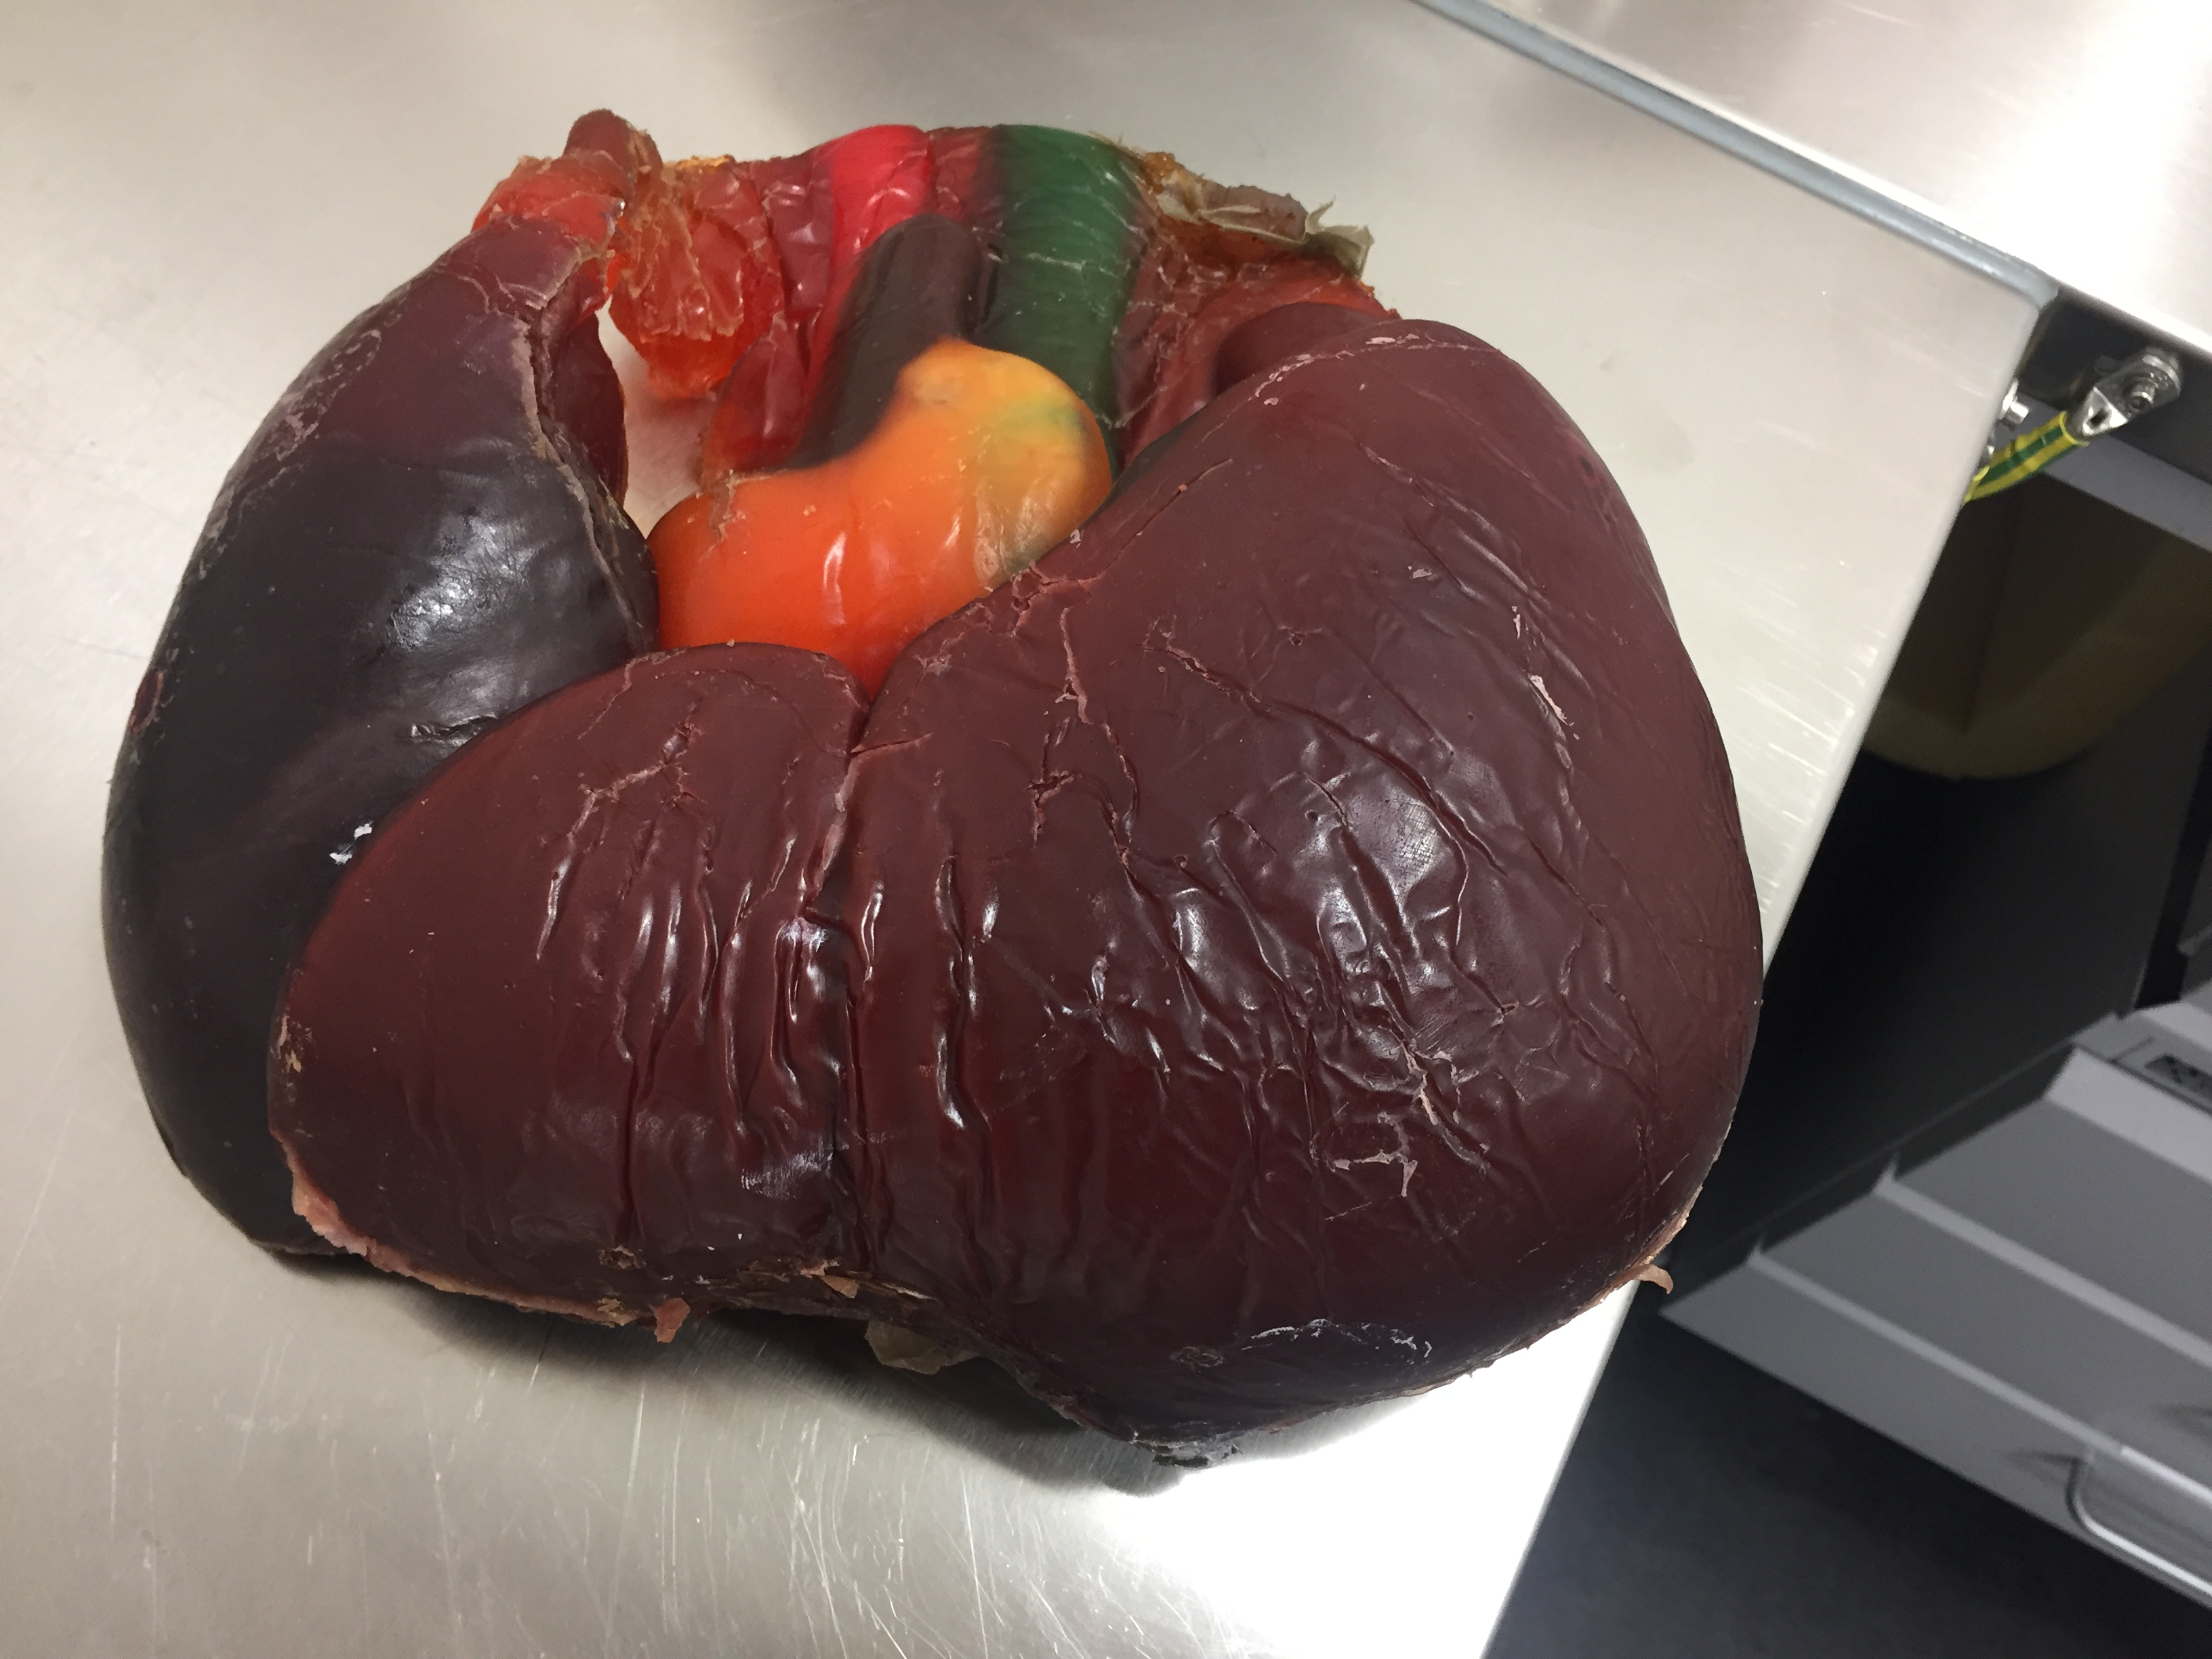
\includegraphics[width=\textwidth]{usedPhantom}
 \caption{The US liver phantom used for the experiments in this study}
  \label{fig:usedPhantom}
\end{figure}

\begin{figure}[H]
  \centering
  \begin{tabular}[H]{c|c|c}
    \addheight{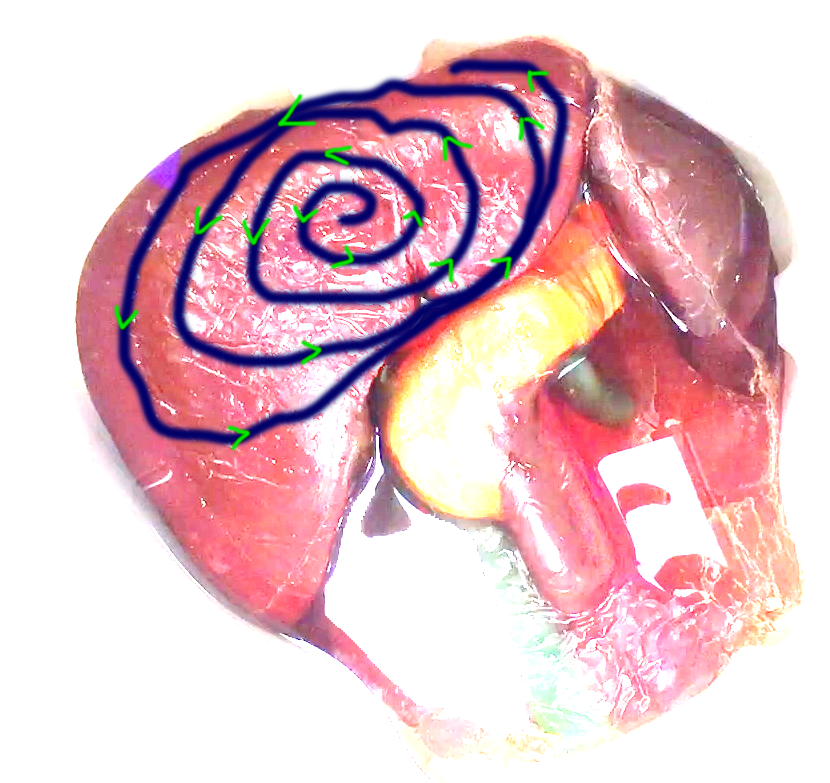
\includegraphics[width=0.3\linewidth]{methods_schnecke_nach_aussen}} &
    \addheight{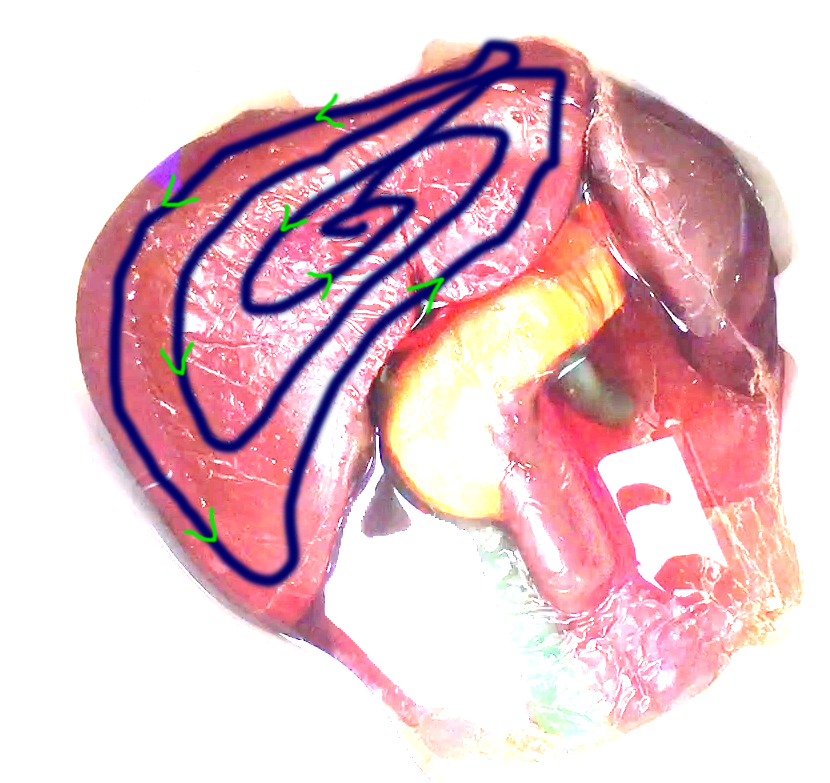
\includegraphics[width=0.3\linewidth]{methods_schnecke_nach_innen}} &
    \addheight{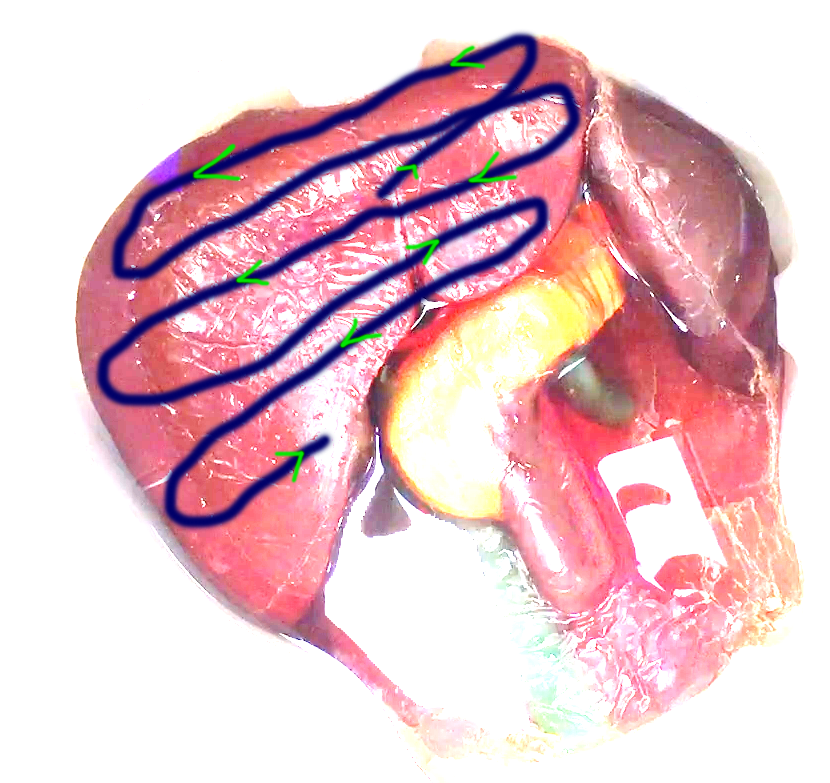
\includegraphics[width=0.3\linewidth]{methods_hin_und_her}}
    \\
    \small Spiral out & Spiral in & Sweep LR
    \\
    \hline
    \addheight{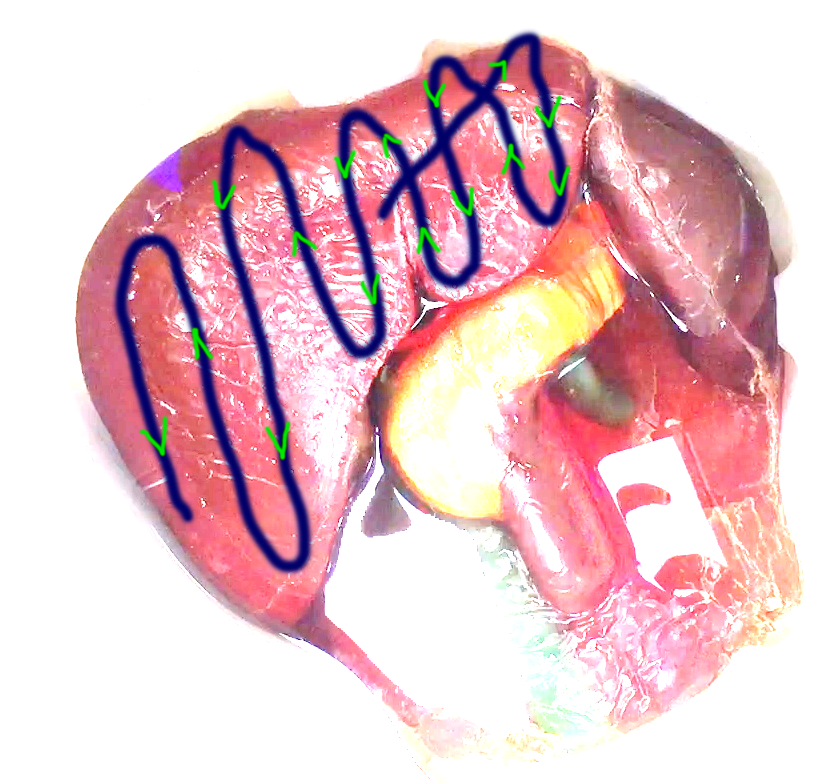
\includegraphics[width=0.3\linewidth]{methods_vor_zurueck}} & 
    \addheight{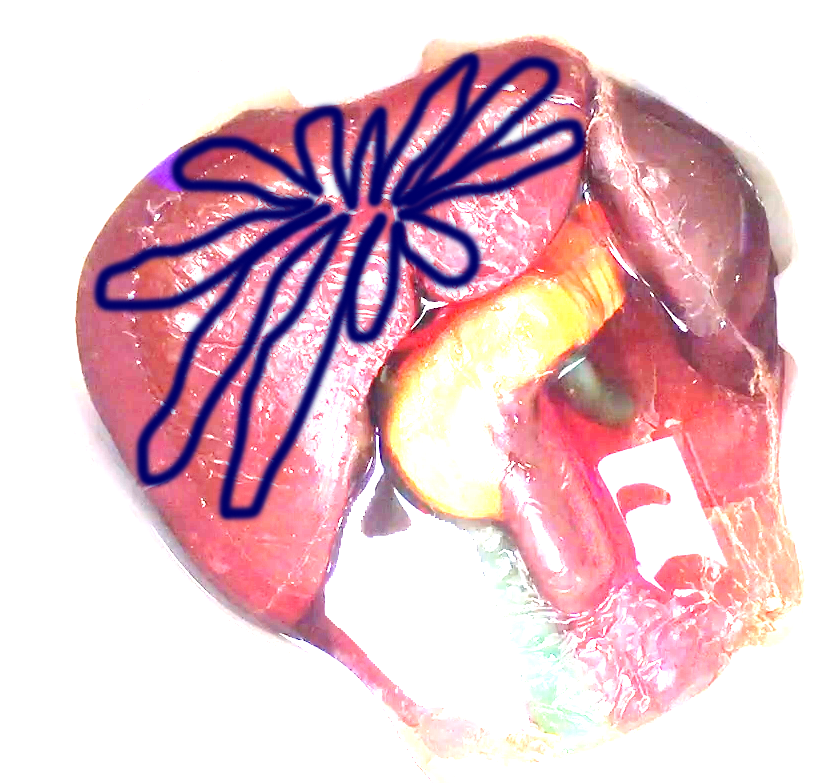
\includegraphics[width=0.3\linewidth]{methods_blume}} &
    \addheight{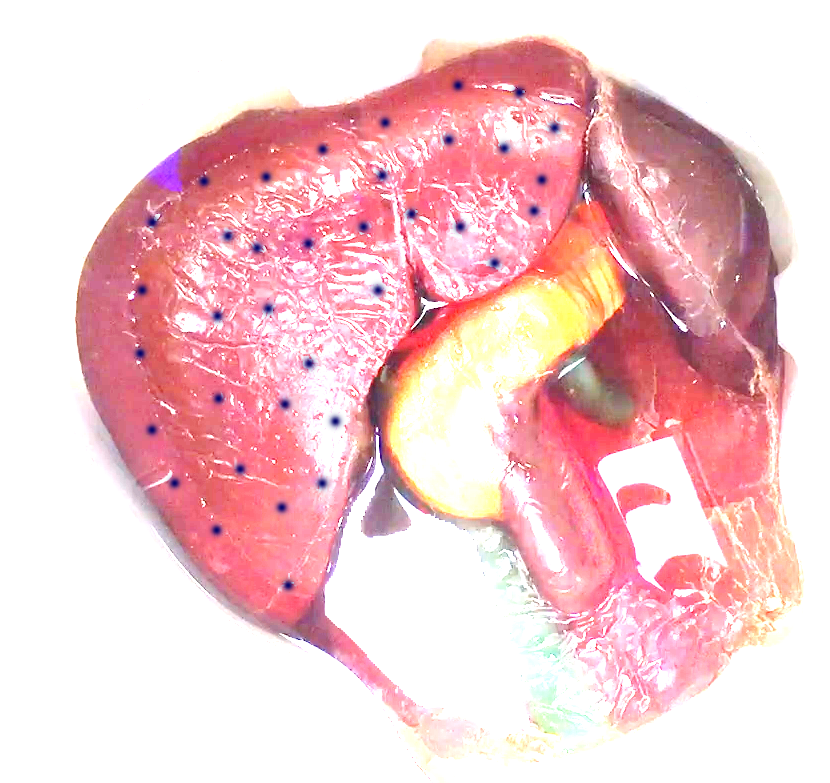
\includegraphics[width=0.3\linewidth]{methods_biene}}
    \\
    \small Sweep FB & Flower & Point grid
    \\
  \end{tabular}
  \caption{Different sampling movements of the ultrasound device over the surface of the liver}
  \label{fig:movements}
\end{figure}

\subsubsection{Surface contact detection}
In the surface contact detection step, a classifier detects whether the US probe
has contact to the liver or not. Therefore, a support vector machine (SVM) was
trained with US images from the phantom and from previous navigated liver
surgeries. The SVM was trained to classify the image into “no surface contact”
(left) and “surface contact” (middle and right). The images were labelled as
“surface contact” if at least 50\% and the center had contact to the surface
(Figure \ref{fig:contactVSnocontact}  middle).  The classifier takes into account that US waves are reflected
at the US probe-air interface when the US probe has no contact to the liver and
therefore no image is formed.
The features for the classifier were: mean, median, minimum, maximum, variance,
skewness and kurtosis of the pixel values. All features are calculated on the
upper half of the image. For training, a set of 2’311 images (1’056 with
contact, 1’255 without contact) were used. The training data was composed of
images from a phantom (88\%) and images from previous navigated liver surgeries
(12\%). All computations were performed using the SciPy software package.


\subsubsection{Surface reconstruction}
To reconstruct the surface of the liver from the sampled points, the surface
reconstruction algorithm by Hoppe et al. \cite{hoppe1992surface}  was used. The algorithm consists
of three phases. From an unorganized set of points, phase 1 constructs an
initial dense mesh. Starting with the dense mesh created in phase 1, phase 2
reduces the number of faces and improves the fit to the data points. In phase 3,
the surface representation is changed from a piecewise linear one (meshes) to a
piecewise smooth one. For the computations the implementation in VTK
(SurfaceReconstructionFilter) was used (neighborhood size of 50 and sample
spacing of 10). Due to the different latencies of the US and the tracking system
(with the US being slower), a delay of 4 frames (0.2 seconds) is applied to the
tracking data.

\subsubsection{Experimental evaluation}
For evaluation of the surface detector the data was split into training (80\%)
and test data (20\%). The precision and recall were calculated for performance
analysis on the test set. To quantitatively evaluate the reconstructed surfaces,
the points of the point grid measurement (414 points) were used as a reference.
These reference points represent points on the surface of the liver in an
undeformed state. For each of these reference points, the error is computed as
the shortest distance to the reconstructed surface. All computations were
performed using SciPy.

\subsection{Results}
Overall, the surface contact detector was evaluated on a test set with 2414
images. Additionally, 10 scans of the liver surface were evaluated against the
reference points to measure the accuracy of the surface reconstruction.

\subsubsection{Surface contact detection}
To evaluate the contact detector, a test set of 2414 images with 50\% contact
and 50\% no contact was used. The detector has a sensitivity of 0.95 and a
specificity of 0.98. Out of all negative samples, 1.9\% were detected as having
contact. The prediction of one image takes 15 ms where most of the time (approx.
99\%) is spent for feature extraction.

\subsubsection{Surface reconstruction}
\textbf{Visual assessment}

The reconstruction of the liver surface created lead to a smoothed version of
the measured surface part. The measured surface corresponds to the surface of
the liver (Figure \ref{fig:usedPhantom}). However, the reconstructed surface area is larger than the
sampled part of the surface. This is a property of the algorithm, as it
estimates a rectangular grid.
\begin{figure}[H]
  \centering
  \begin{tabular}[H]{c|c|c}
    \addheight{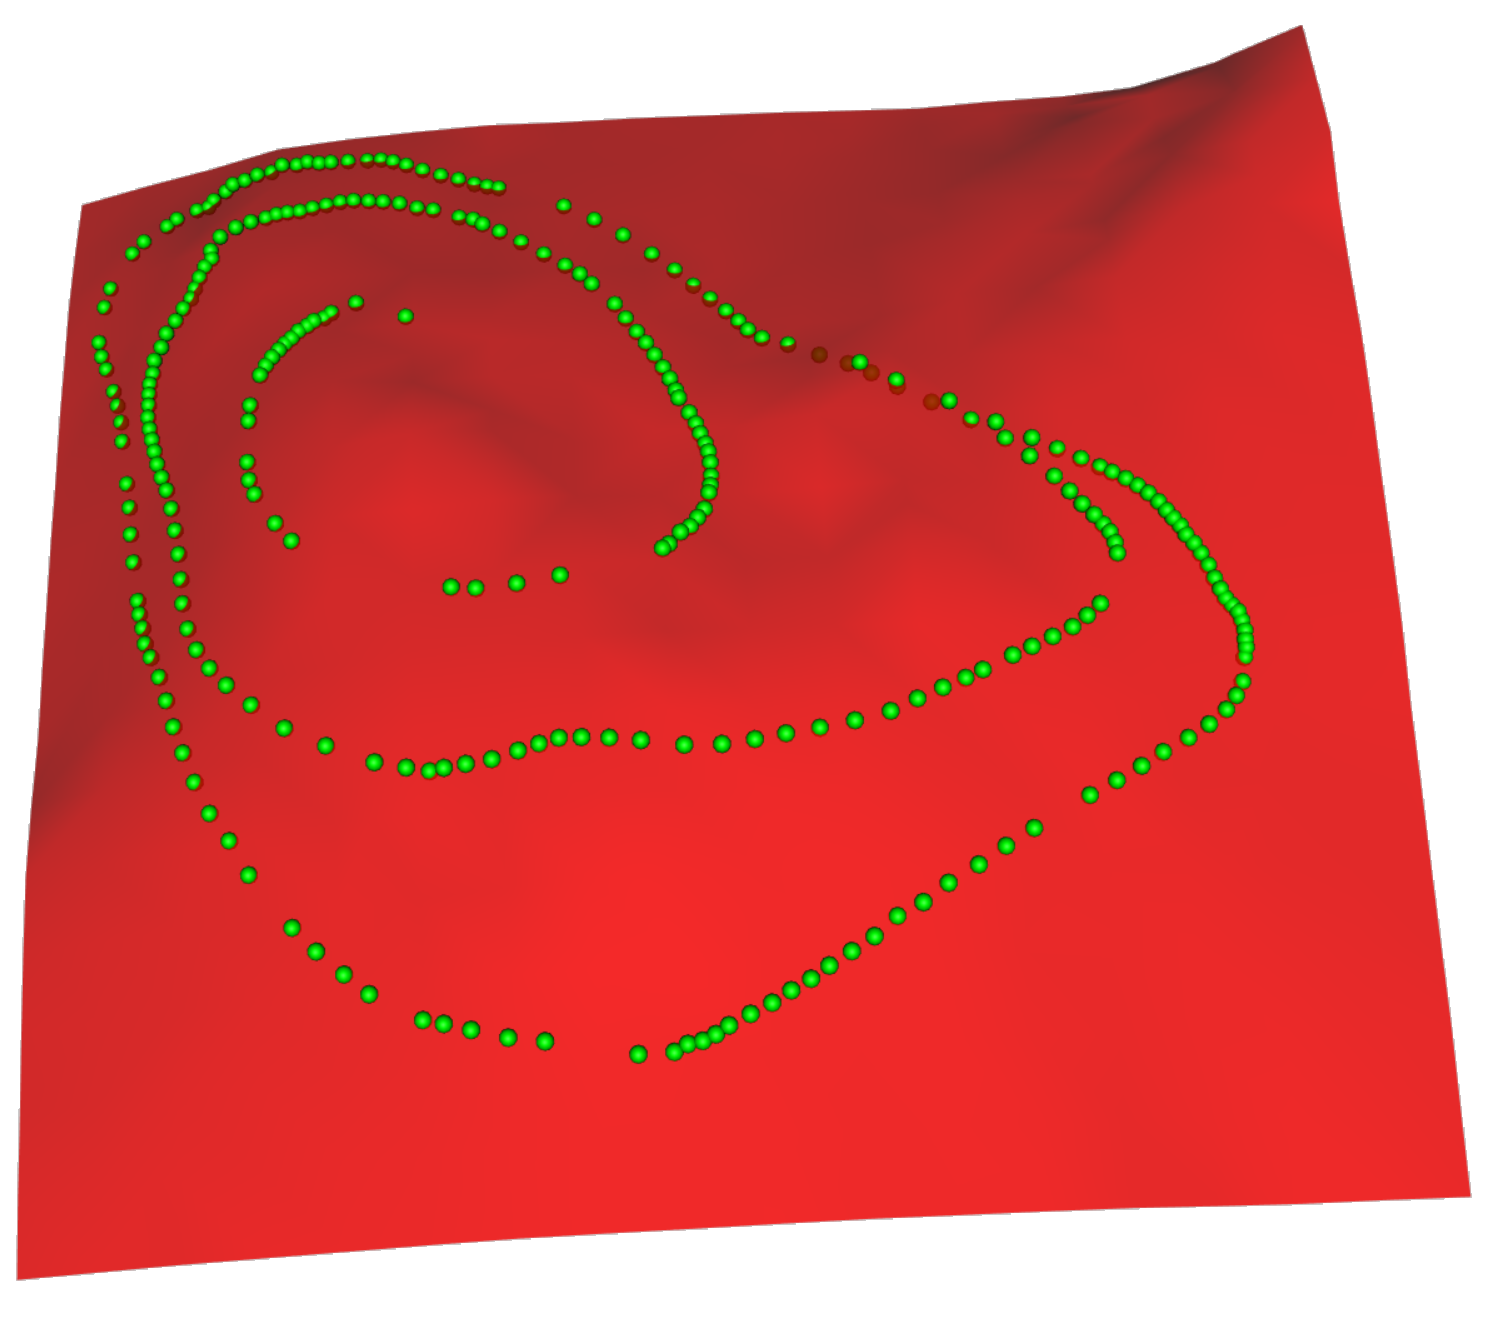
\includegraphics[width=0.3\linewidth]{mes05_spiral_out.png}} &
    \addheight{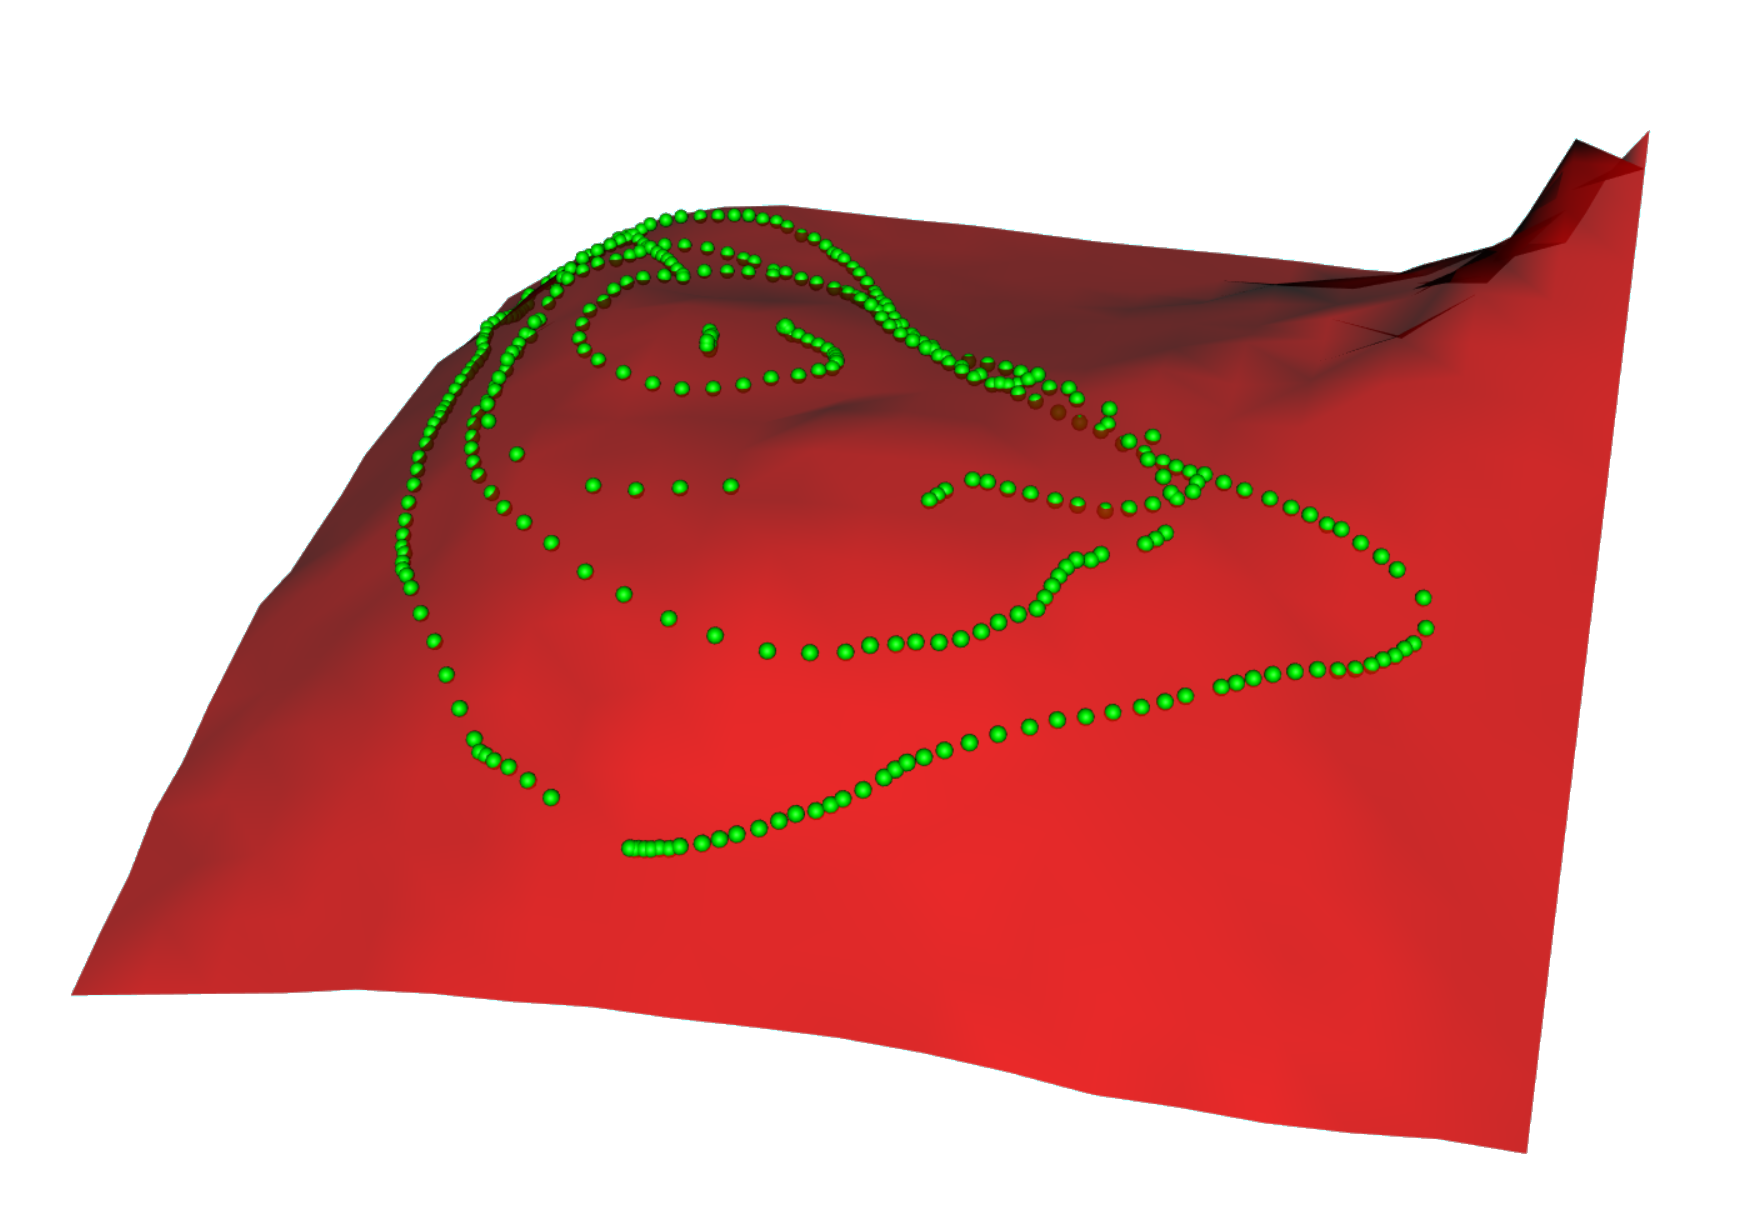
\includegraphics[width=0.3\linewidth]{mes03_spiral_in.png}} &
    \addheight{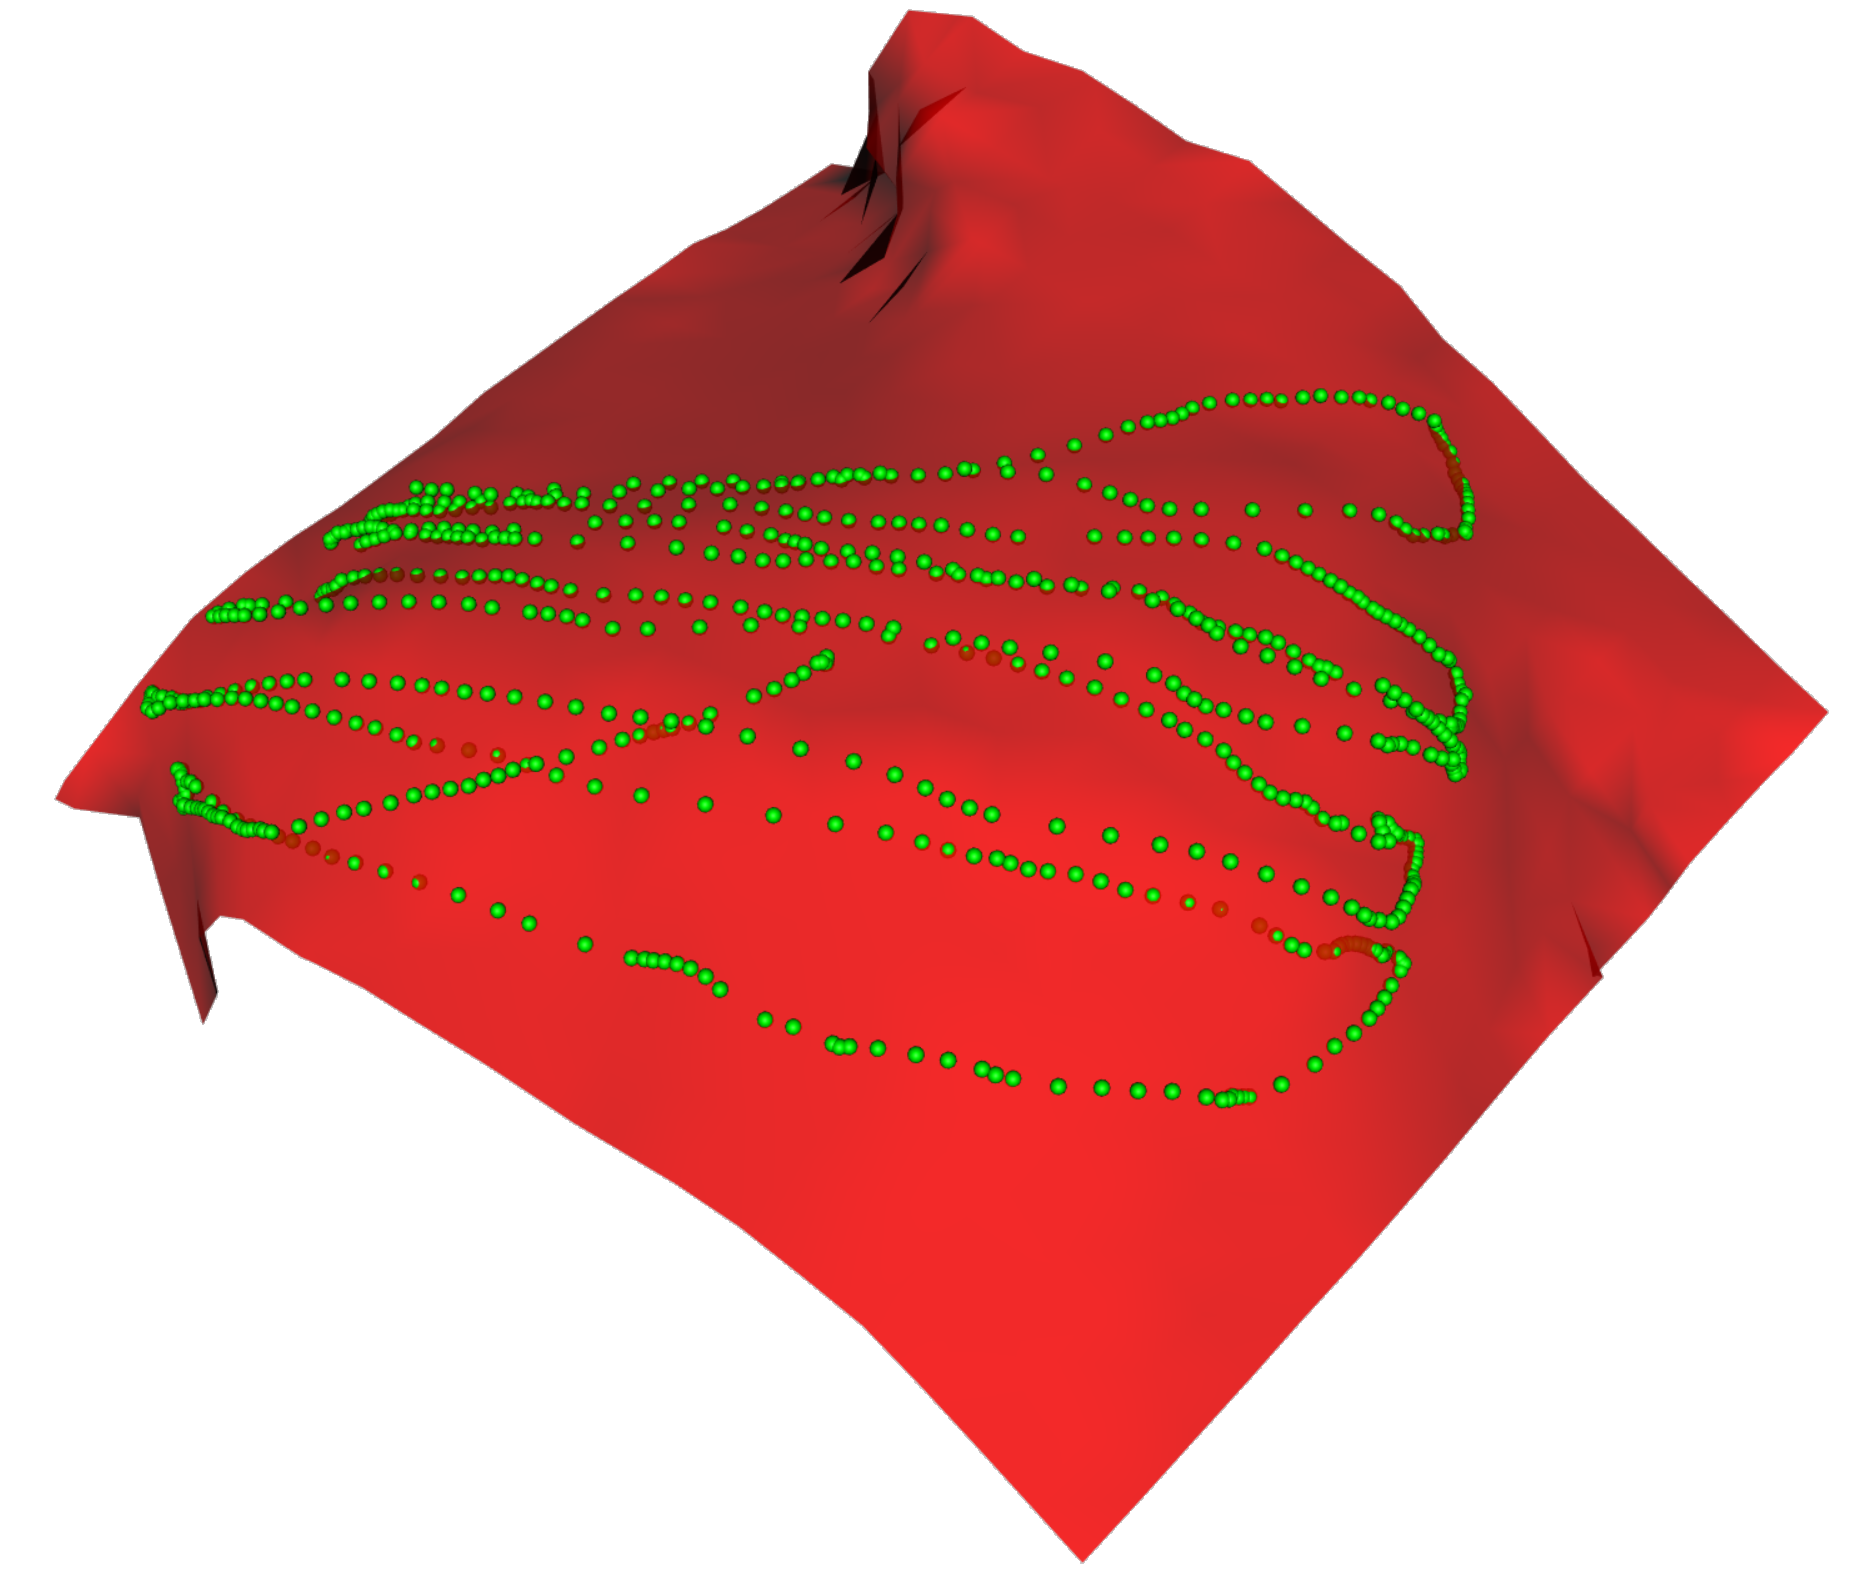
\includegraphics[width=0.3\linewidth]{mes11_sweepLR.png}}
    \\
    \small Spiral out & Spiral in & Sweep LR
    \\
    \hline
    \addheight{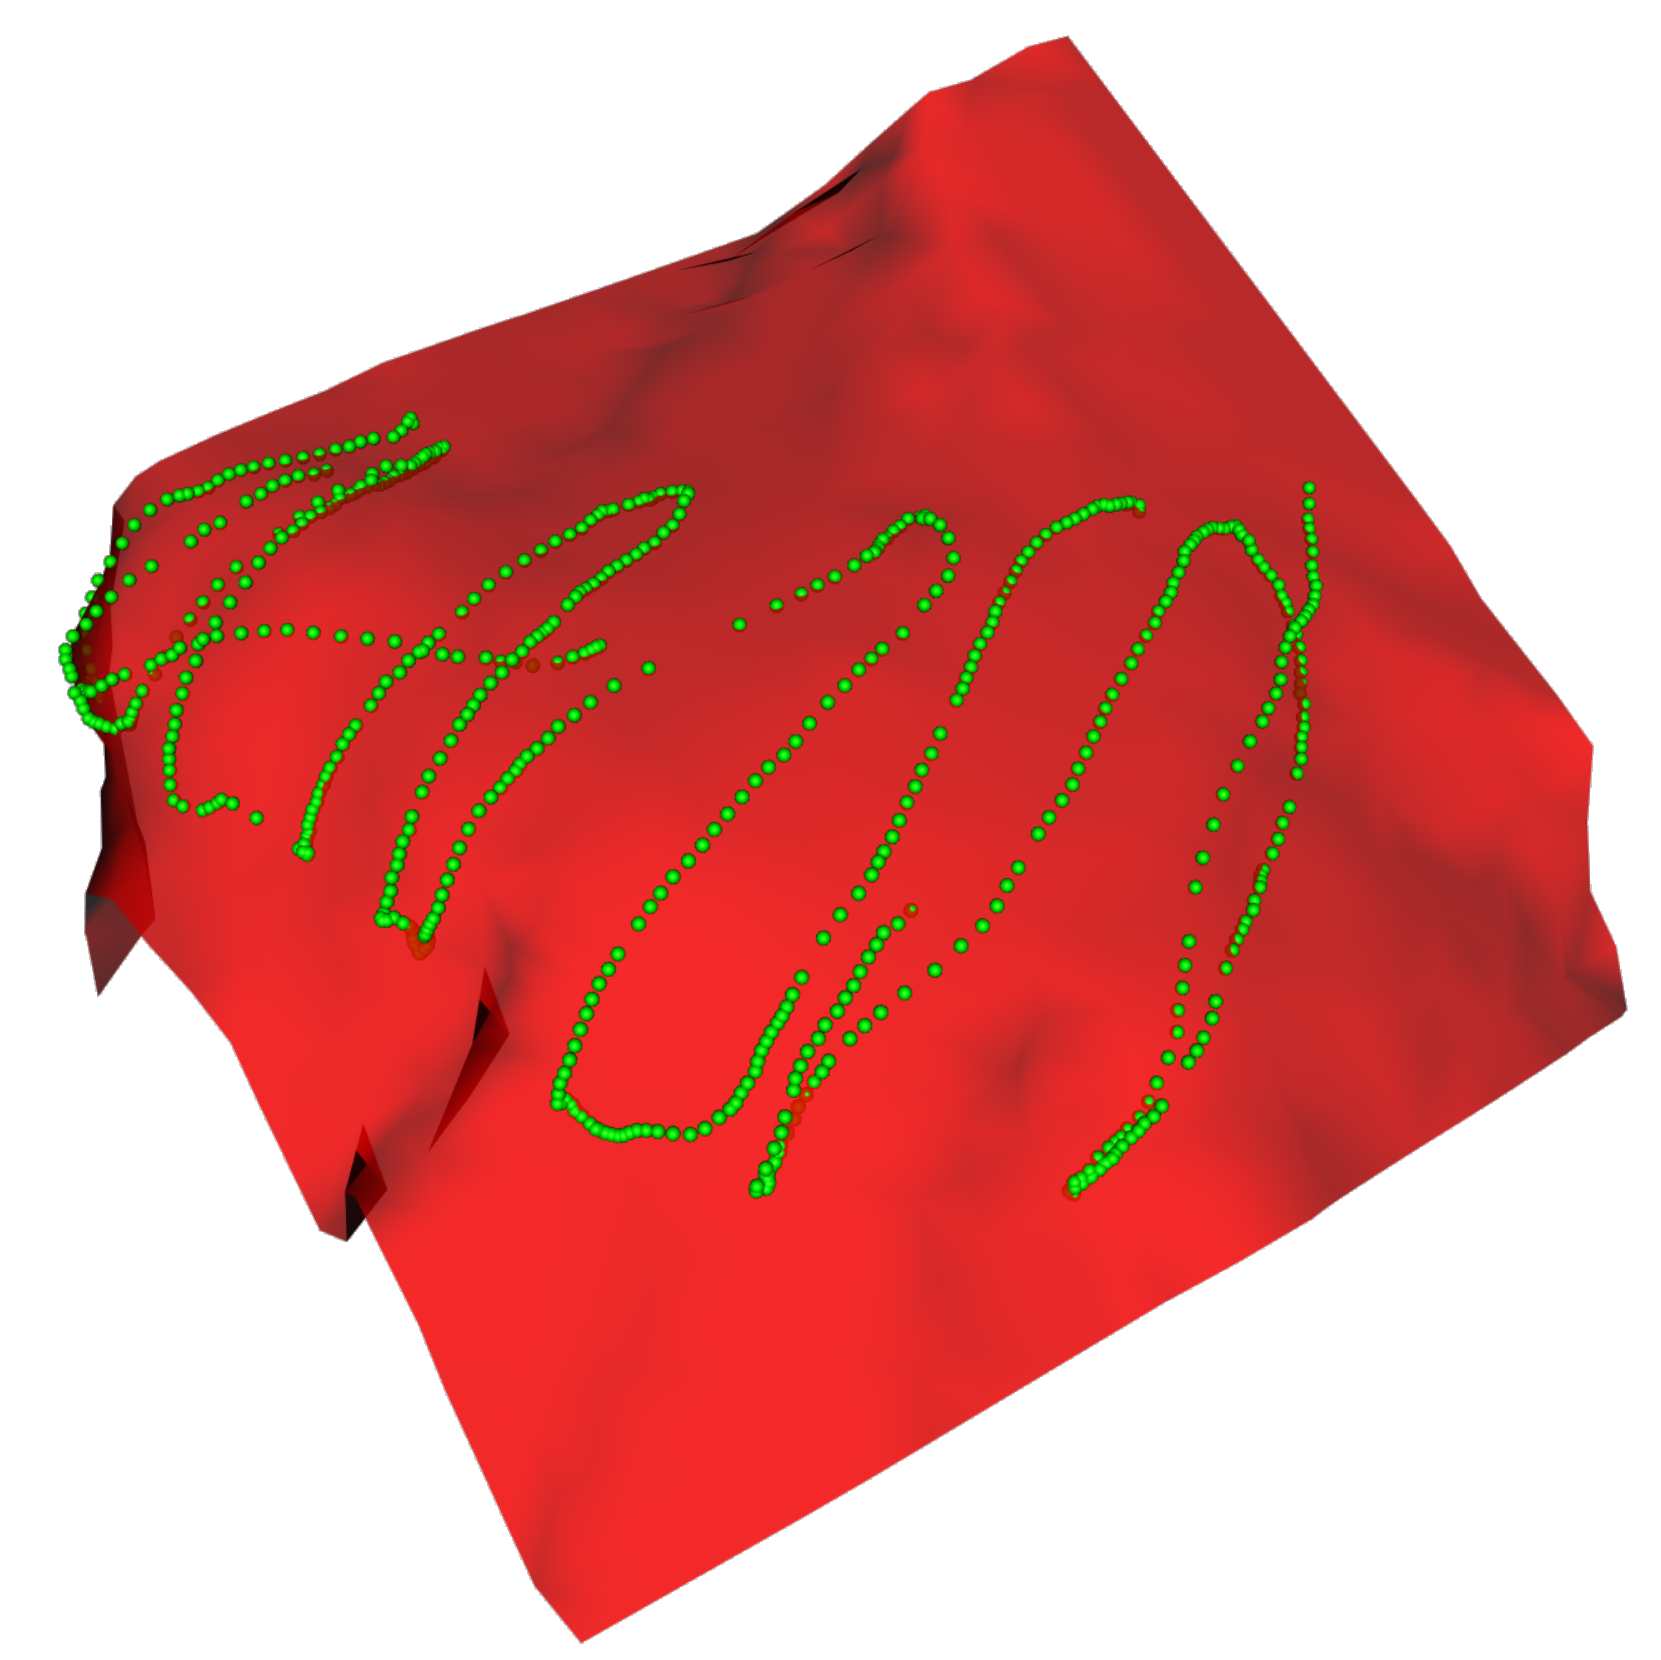
\includegraphics[width=0.3\linewidth]{mes12_sweepFB.png}} &
    \addheight{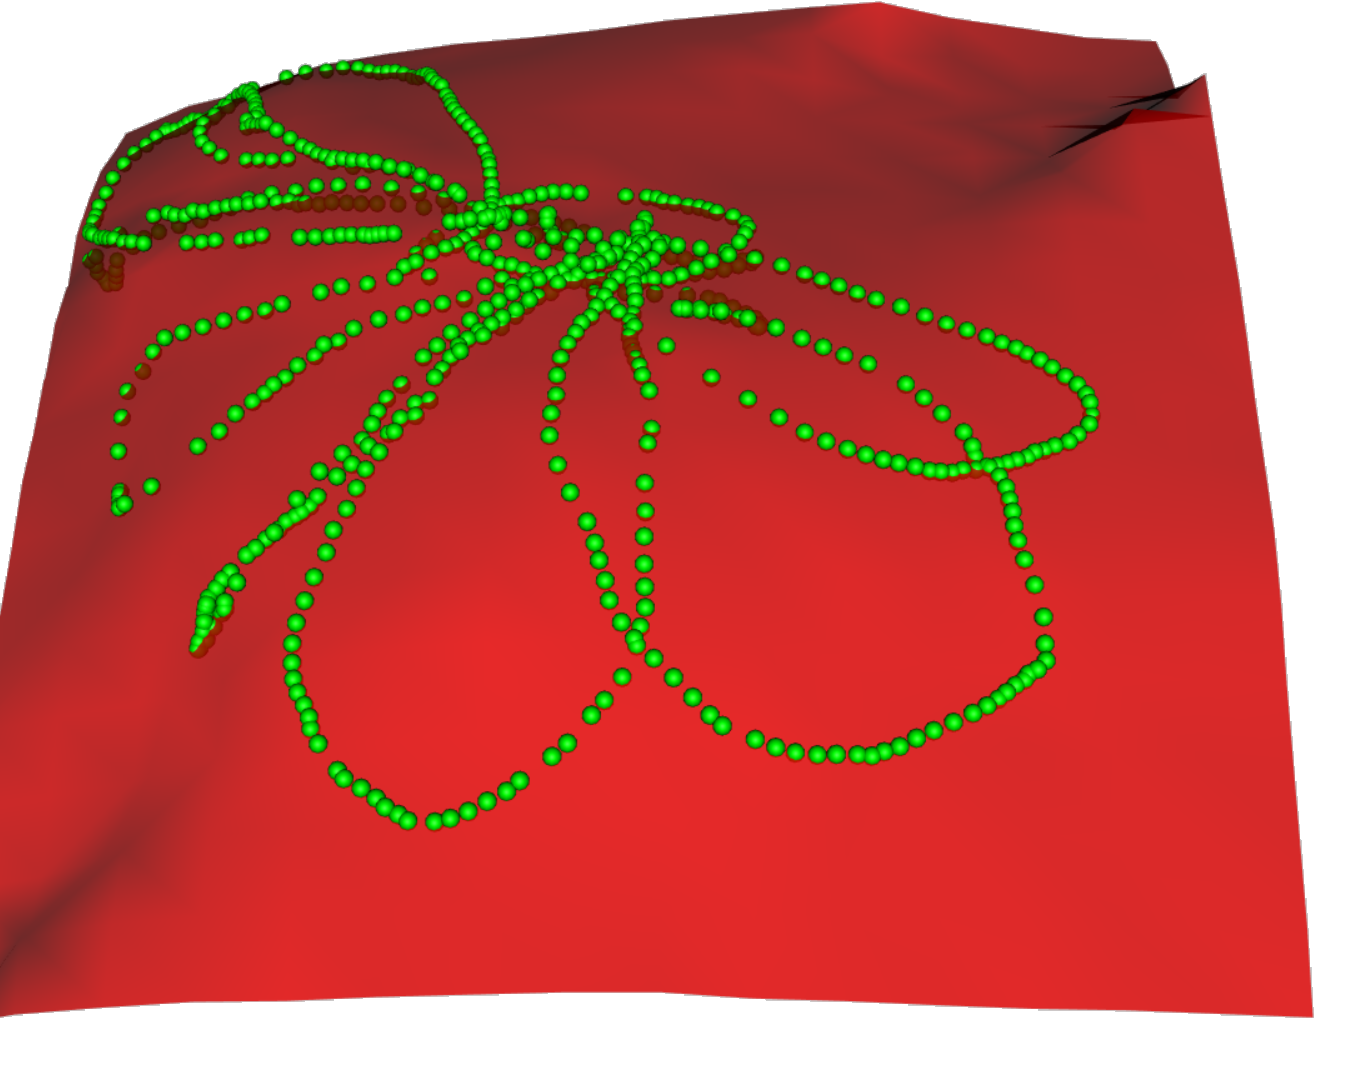
\includegraphics[width=0.3\linewidth]{mes07_flower.png}} &
    \addheight{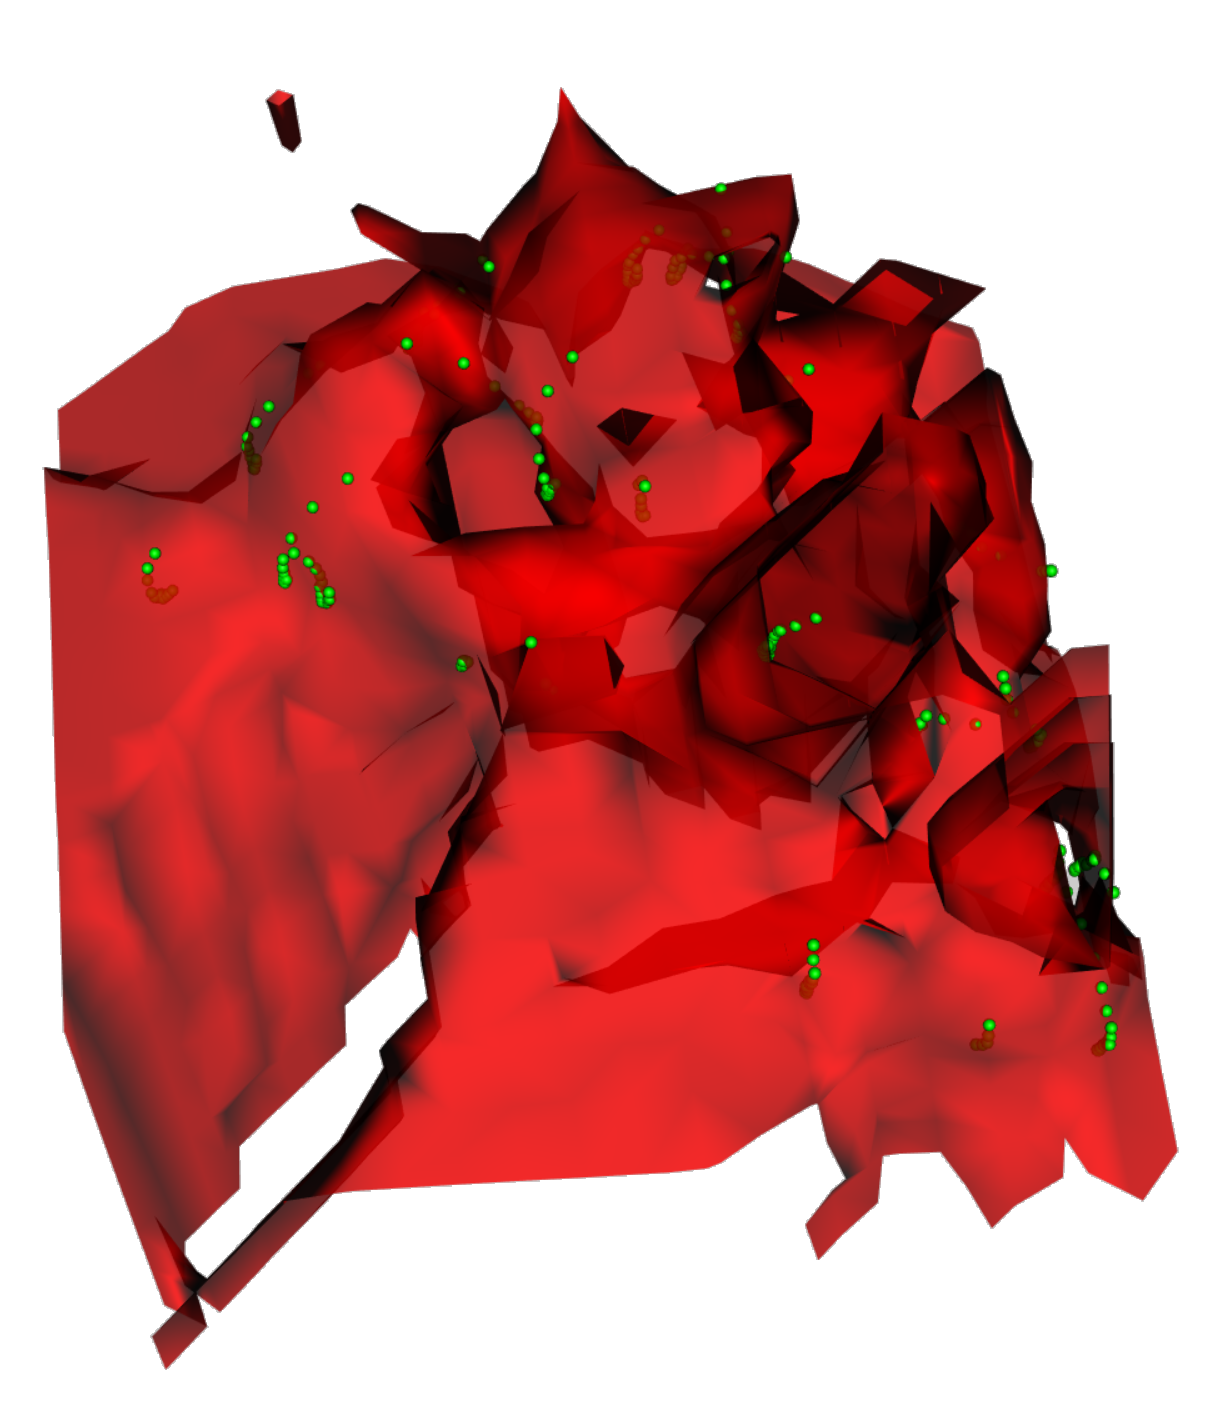
\includegraphics[width=0.3\linewidth]{mes08_pointgrid.png}}
    \\
    \small Sweep FB & Flower & Point grid
    \\
  \end{tabular}
  \caption{Reconstructed surfaces from different movements of the ultrasound device over the
    surface of the liver model. The names correspond to the movement drawings in figure \ref{fig:movements}}
  \label{fig:soft_liver_movements}
\end{figure}
\textbf{Quantitative analysis}

To evaluate the accuracy of the reconstructed surfaces, the shortest distance of
the reference points to the surface were computed. The overall median error for all the measurements is 2,5mm with an
interquartile range of 1 mm – 5 mm. By projecting these errors corresponding to
each reference point onto the liver surface, one can see that the highest errors
are in segments 2 and 3 And the lowest in segments 4, 5, 6 and 8 (Figure \ref{fig:surfaceErrors}).

\begin{figure}[H]
  \centering
 \includegraphics[width=\textwidth]{surfaceErrors}
 \caption{The mean distance of each reference point visualized by colors. All
   points with a mean distance of over 5 mm to the surface are colored dark red.
   Points with a mean distacne below 1.5 mm are colored dark green.}
  \label{fig:surfaceErrors}
\end{figure}

\subsection{Discussion}
The surface contact detector is correctly classifying in 96\% of the cases, with
a very low false positive rate of 1.9\%. This is especially important, as false
positives lead to artifacts in the reconstructed surface. Furthermore, the
processing time of 15 ms per image makes it suitable for real-time processing of
the images as the ultrasound scanner runs at 20 Hz (50 ms / frame). When the US
probe is removed from the liver surface there are 3-5 images which are wrongly
classified as having a signal. This would cause artifacts in the surface
reconstruction, and therefore they are filtered out later for surface
reconstruction. This is mainly, because of the latency of the US scanner itself
compared to the tracking system. The images are slightly blurrier (Figure \ref{fig:classificationProblem}), but
from the tracking positions one can clearly see that they are not on the
surface.

% \begin{figure}[H]
%   \centering
%  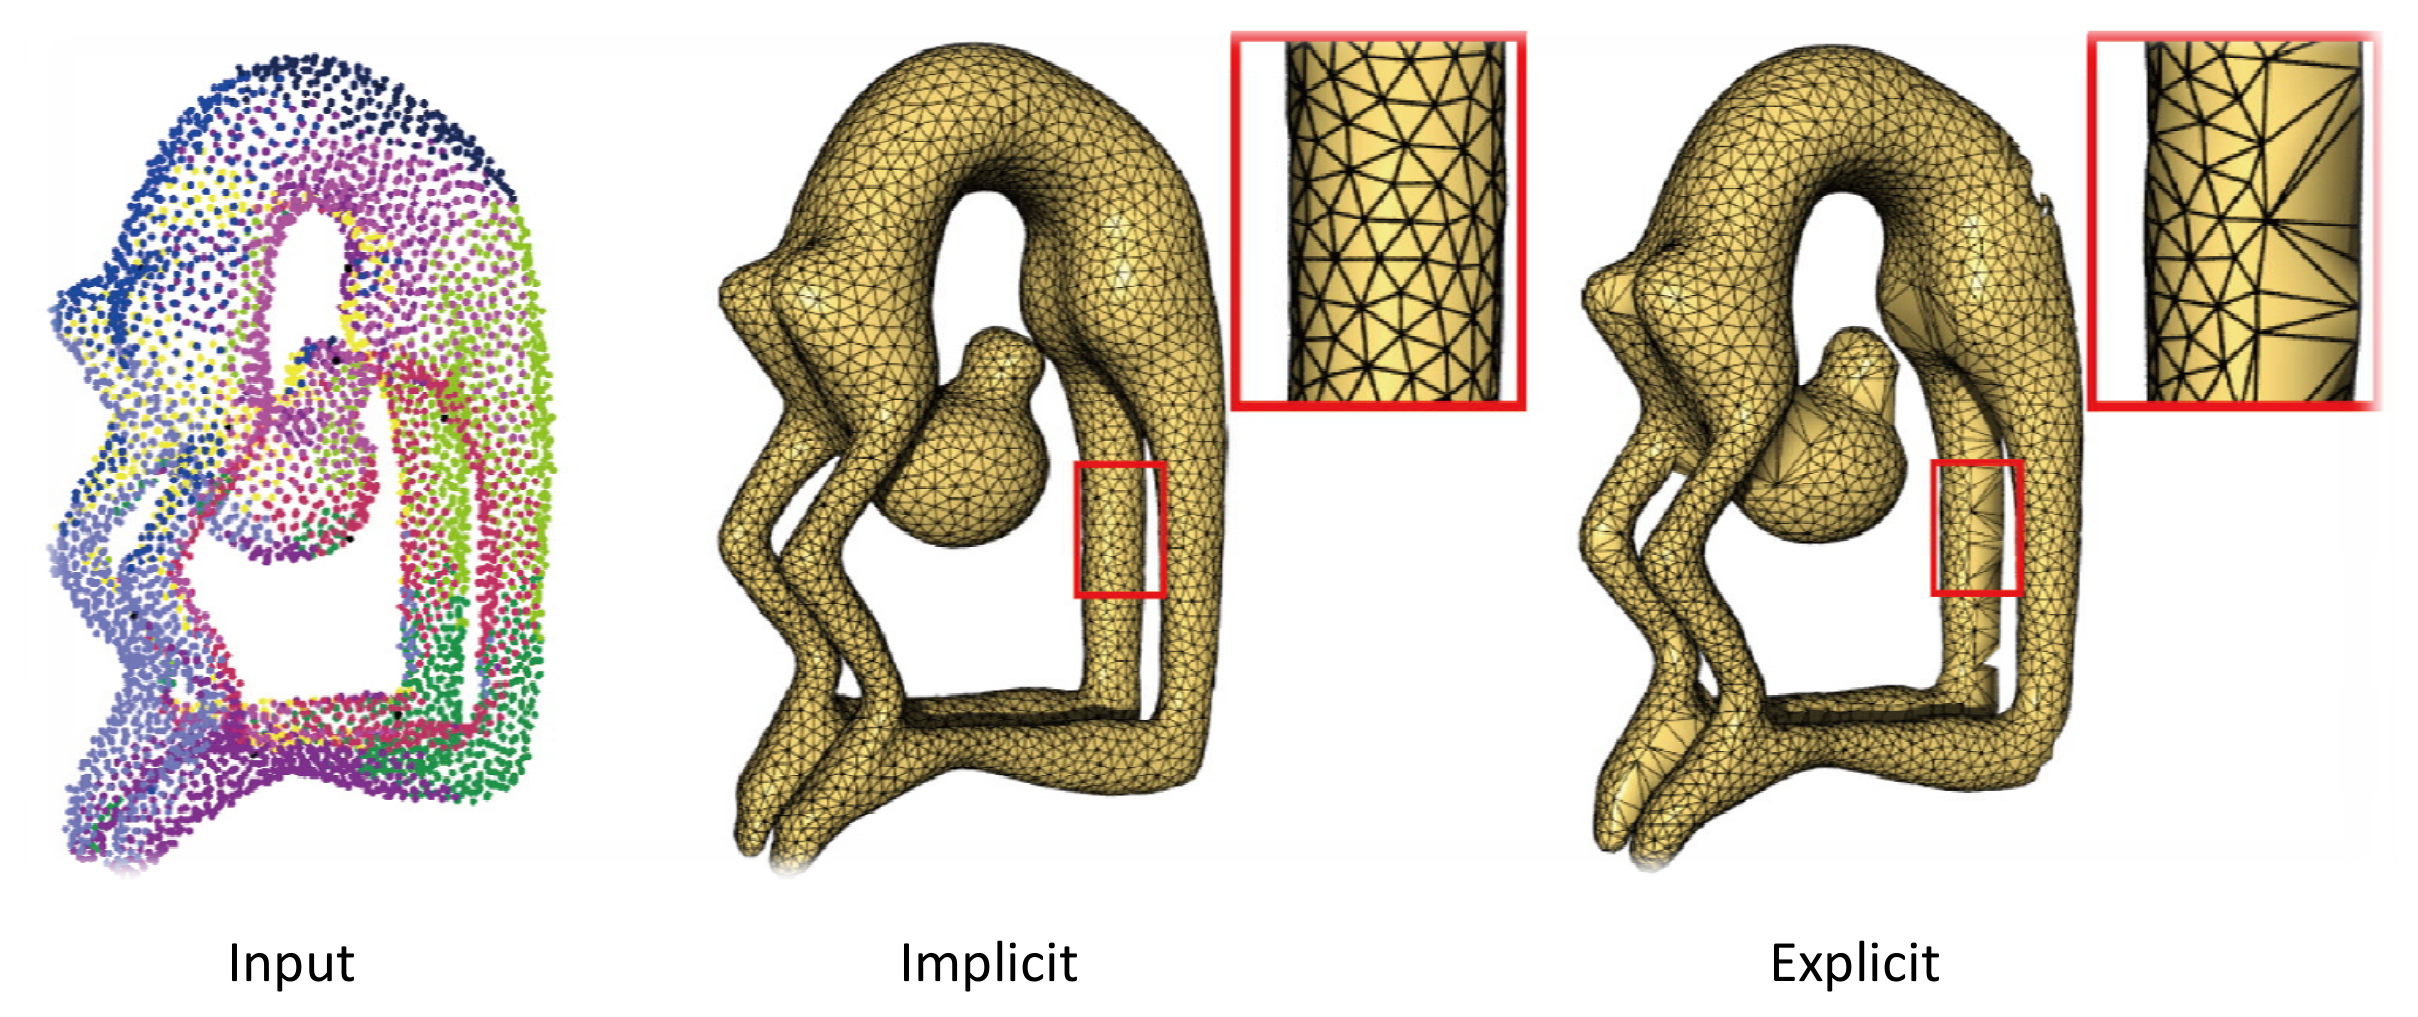
\includegraphics[width=\textwidth]{ImplicitVSExplicit}
%  \caption{Wrong and correct classified images at the end of the measurement}
%   \label{fig:ImplicitVSExplicit}
% \end{figure}

\begin{figure}[H]
  \centering
  \minipage{0.32\linewidth}
    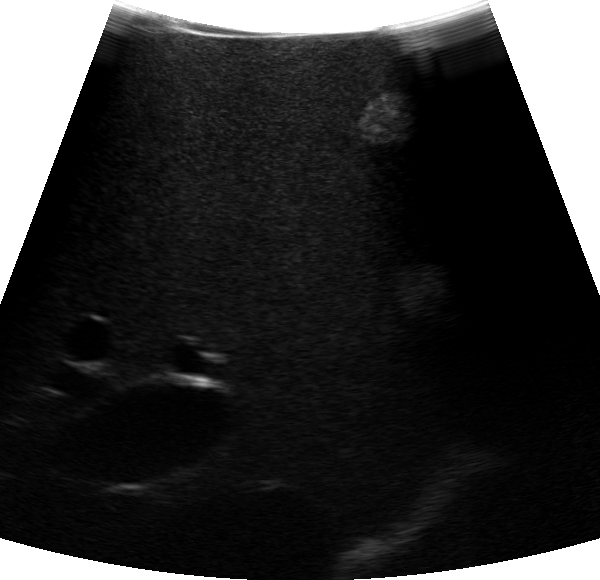
\includegraphics[width=\linewidth]{wrong_classified}
  \endminipage
  \minipage{0.1\linewidth}
  \hfill
  \endminipage
  \minipage{0.32\linewidth}
    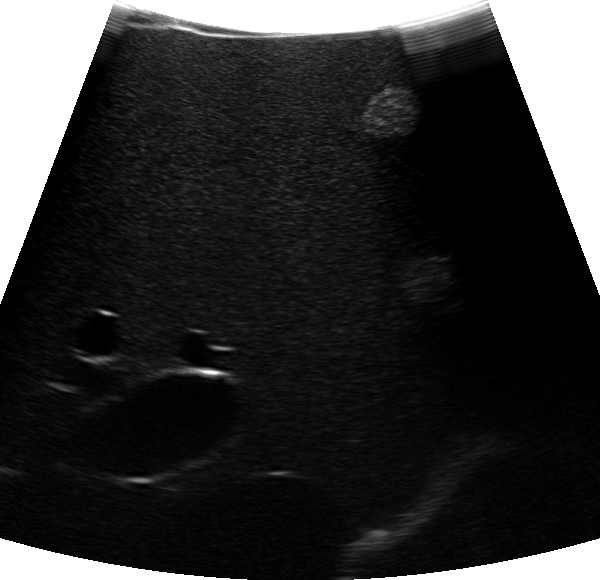
\includegraphics[width=\linewidth]{correct_classified}
  \endminipage
  \caption{Wrong and correct classified images at the end of the measurement}
  \label{fig:classificationProblem}
\end{figure}

\subsubsection{Surface reconstruction}
From a visual point of view the reconstructed surfaces of the US liver phantom
look similar to the surface of the liver model. However, the spiral and the
flower movement, led to a more accurate reconstruction.

From a quantitative point of view, it turned out that the largest average errors
are in segment 2 and 3. This is likely because these liver segments are the
softest on the phantom used for the measurements. Due to that, this segment was
pressed down during the measurement which lead to a surface with a large
distance to the reference points. Additionally, one can see that the average
distance at the boundary of the liver is large as well. This could be because
the US device was held between the wall of the tank and the liver model. Because
of the small space between the wall and the liver, the pressure applied on the
liver was larger than in other areas and the consequent distance between the
reference points and the deformed surface became larger. However, this might
also be the case in a clinical setting, as these regions are more difficult to
reach with the US probe. Overall, the best accuracy, could be achieved in
segments 4,5,6 and 8, which were the easiest to access in this setup. In a next
step, this would also be analyzed on the human liver, to see in which segments
this technique can be applied accurately.

To conclude, we presented a surface reconstruction technique, which can be used
to intraoperatively acquire a surface model of the liver using navigated US.
This can then be further used for intraoperative resection planning or
surface-based registration.


\section{Surface reconstruction on retrospective data}
\subsection{Methodology}
Retrospective data from Banz et. al
\subsection{Results}
\subsection{Discussion}

\section{Usability Test}
3 surgeons
questionnaire
surface accuracy (using surface registration)
\subsection{Methodology}
\subsection{Results}
\subsection{Discussion}
%%% Local Variables:
%%% TeX-master: "MscThesis"
%%% End: